%%%%%%%%%%%%%%%%%%%%%%%%%%%%%%%%%%%%%%%%%
% Beamer Presentation
% LaTeX Template
% Version 1.0 (10/11/12)
%
% This template has been downloaded from:
% http://www.LaTeXTemplates.com
%
% License:
% CC BY-NC-SA 3.0 (http://creativecommons.org/licenses/by-nc-sa/3.0/)
%
%%%%%%%%%%%%%%%%%%%%%%%%%%%%%%%%%%%%%%%%%

%----------------------------------------------------------------------------------------
%	PACKAGES AND THEMES
%----------------------------------------------------------------------------------------

\documentclass[]{beamer}

\mode<handout>
{
  \usepackage{pgf}
  \usepackage{pgfpages}

\pgfpagesdeclarelayout{4 on 1 boxed}
{
  \edef\pgfpageoptionheight{\the\paperheight} 
  \edef\pgfpageoptionwidth{\the\paperwidth}
  \edef\pgfpageoptionborder{0pt}
}
{
  \pgfpagesphysicalpageoptions
  {%
    logical pages=4,%
    physical height=\pgfpageoptionheight,%
    physical width=\pgfpageoptionwidth%
  }
  \pgfpageslogicalpageoptions{1}
  {%
    border code=\pgfsetlinewidth{2pt}\pgfstroke,%
    border shrink=\pgfpageoptionborder,%
    resized width=.5\pgfphysicalwidth,%
    resized height=.5\pgfphysicalheight,%
    center=\pgfpoint{.25\pgfphysicalwidth}{.75\pgfphysicalheight}%
  }%
  \pgfpageslogicalpageoptions{2}
  {%
    border code=\pgfsetlinewidth{2pt}\pgfstroke,%
    border shrink=\pgfpageoptionborder,%
    resized width=.5\pgfphysicalwidth,%
    resized height=.5\pgfphysicalheight,%
    center=\pgfpoint{.75\pgfphysicalwidth}{.75\pgfphysicalheight}%
  }%
  \pgfpageslogicalpageoptions{3}
  {%
    border code=\pgfsetlinewidth{2pt}\pgfstroke,%
    border shrink=\pgfpageoptionborder,%
    resized width=.5\pgfphysicalwidth,%
    resized height=.5\pgfphysicalheight,%
    center=\pgfpoint{.25\pgfphysicalwidth}{.25\pgfphysicalheight}%
  }%
  \pgfpageslogicalpageoptions{4}
  {%
    border code=\pgfsetlinewidth{2pt}\pgfstroke,%
    border shrink=\pgfpageoptionborder,%
    resized width=.5\pgfphysicalwidth,%
    resized height=.5\pgfphysicalheight,%
    center=\pgfpoint{.75\pgfphysicalwidth}{.25\pgfphysicalheight}%
  }%
}


  \pgfpagesuselayout{4 on 1 boxed}[a4paper, border shrink=5mm, landscape]
  \nofiles
}

\mode<presentation> {

% The Beamer class comes with a number of default slide themes
% which change the colors and layouts of slides. Below this is a list
% of all the themes, uncomment each in turn to see what they look like.

%\usetheme{default}
%\usetheme{AnnArbor}
%\usetheme{Antibes}
%\usetheme{Bergen}
%\usetheme{Berkeley}
%\usetheme{Berlin}
%\usetheme{Boadilla}
\usetheme{CambridgeUS}
%\usetheme{Copenhagen}
%\usetheme{Darmstadt}
%\usetheme{Dresden}
%\usetheme{Frankfurt}
%\usetheme{Goettingen}
%\usetheme{Hannover}
%\usetheme{Ilmenau}
%\usetheme{JuanLesPins}
%\usetheme{Luebeck}
%\usetheme{Madrid}
%\usetheme{Malmoe}
%\usetheme{Marburg}
%\usetheme{Montpellier}
%\usetheme{PaloAlto}
%\usetheme{Pittsburgh}
%\usetheme{Rochester}
%\usetheme{Singapore}
%\usetheme{Szeged}
%\usetheme{Warsaw}

% As well as themes, the Beamer class has a number of color themes
% for any slide theme. Uncomment each of these in turn to see how it
% changes the colors of your current slide theme.

%\usecolortheme{albatross}
%\usecolortheme{beaver}
%\usecolortheme{beetle}
%\usecolortheme{crane}
\usecolortheme{dolphin}
%\usecolortheme{dove}
%\usecolortheme{fly}
%\usecolortheme{lily}
%\usecolortheme{orchid}
%\usecolortheme{rose}
%\usecolortheme{seagull}
%\usecolortheme{seahorse}
%\usecolortheme{whale}
%\usecolortheme{wolverine}

%\setbeamertemplate{footline} % To remove the footer line in all slides uncomment this line
%\setbeamertemplate{footline}[page number] % To replace the footer line in all slides with a simple slide count uncomment this line

%\setbeamertemplate{navigation symbols}{} % To remove the navigation symbols from the bottom of all slides uncomment this line
}

\usepackage{graphicx} % Allows including images
\usepackage{booktabs} % Allows the use of \toprule, \midrule and \bottomrule in tables
\usepackage[vlined]{algorithm2e}
\usepackage{caption}
\usepackage{subcaption}


%----------------------------------------------------------------------------------------
%	TITLE PAGE
%----------------------------------------------------------------------------------------

\title[Grand Challenge 2015]{DEBS Grand Challenge: A High-Throughput, Scalable Solution for Calculating Frequent Routes and Profitability of New York Taxis} % The short title appears at the bottom of every slide, the full title is only on the title page

\author[Amila Suriarachchi]{Amila Suriarachchi \\ Shrideep Pallickara } % Your name
\institute[CSU] % Your institution as it will appear on the bottom of every slide, may be shorthand to save space
{
Colorado State University \\ % Your institution for the title page
\medskip
\textit{amilas@cs.colostate.edu} % Your email address
\medskip
}
\date{\today} % Date, can be changed to a custom date

\begin{document}

\begin{frame}
\titlepage % Print the title page as the first slide
\end{frame}

\begin{frame}
\frametitle{Outline} % Table of contents slide, comment this block out to remove it
\tableofcontents % Throughout your presentation, if you choose to use \section{} and \subsection{} commands, these will automatically be printed on this slide as an overview of your presentation
\end{frame}

%----------------------------------------------------------------------------------------
%	PRESENTATION SLIDES
%----------------------------------------------------------------------------------------

%------------------------------------------------
\section{Introduction} % Sections can be created in order to organize your presentation into discrete blocks, all sections and subsections are automatically printed in the table of contents as an overview of the talk
%------------------------------------------------

\begin{frame}
\frametitle{Problem Characteristics}
\begin{itemize}
	\item The whole dataset contains 173 million records within year 2013
	\item There are 899010 unique routes and 56697 unique cells
	\item 30 minute time window contains around 10000 events assuming equal event distribution
		\begin{itemize}
			\item Thousands of route and cell details need to process with each event
		\end{itemize}
	\item Top ten frequent routes and profitable cells should be calculated whole dataset
		\begin{itemize}
                        \item Dataset can not be simply partitioned 
                \end{itemize}
\end{itemize}

\end{frame}

\begin{frame}
\frametitle{Research Challenges}
\begin{itemize}
	\item Handling thousands of values in real-time
		\begin{itemize}
			\item An algorithm with O(n) time complexity will not scale for thousands. How can we design an algorithm with O(log n) time complexity?
		\end{itemize}
	\item Parallel evaluation
		\begin{itemize}
                        \item Partitioning route sets and cell sets triggers events for subsets, but application requires the events with whole sets. Therefore is it possible to partition data and still generate required results to support parallelism? 
                \end{itemize}
\end{itemize}

\end{frame}

\begin{frame}
\frametitle{Contributions}
\begin{itemize}
        \item We have designed a set of  generic data structures capable of inserting, updating, removing and retrieving top values (order can be defined using a comparator function) with O(log n) time complexity
        \item Using our data structures we have developed an algorithm to find the running median with O(log n) time complexity 
	\item We have developed a scalable parallel evaluation technique to process queries efficiently
\end{itemize}

\end{frame}

\section{Query Implementation}


\begin{frame}
\frametitle{NodeList Data Structure}

\begin{table}
\centering
\begin{tabular}{|l|l|} \hline
Operation Signature & Time Complexity \\ \hline \hline
add(key : Object, value : NodeValue) & O(log n) \\ \hline
get(key : Object) : NodeValue & O(1) \\ \hline
containsKey(key : Object) : boolean & O(1) \\ \hline
remove(key : Object) : NodeValue & O(log n) \\ \hline
decrementPosition(key : Object) & O(log n) \\ \hline
incrementPosition(key : Object) & O(log n) \\ \hline
getTopValues() : List \textless NodeValue \textgreater & O(1) \\ \hline
\end{tabular}
\end{table}

\begin{figure}
        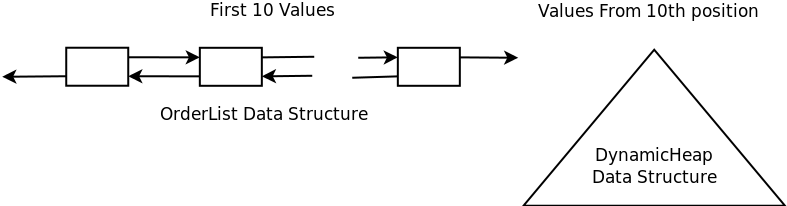
\includegraphics[width=0.8\linewidth]{nodeliststruct.png}
\end{figure}

\end{frame}

\begin{frame}
\frametitle{OrderedList Data Structure}

\begin{figure}
        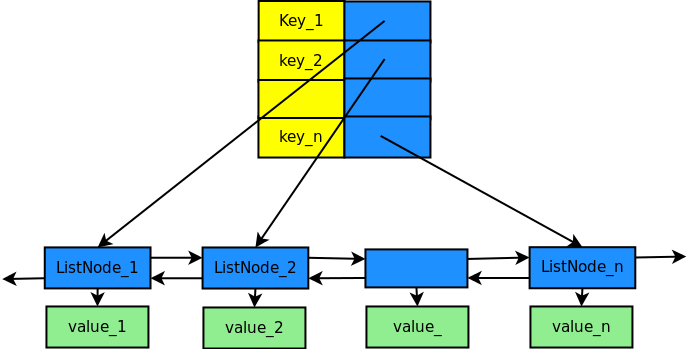
\includegraphics[width=0.8\linewidth]{orderedlist.png}
\end{figure}

\end{frame}

\begin{frame}
\frametitle{DynamicHeap Data Structure}

\begin{figure}
        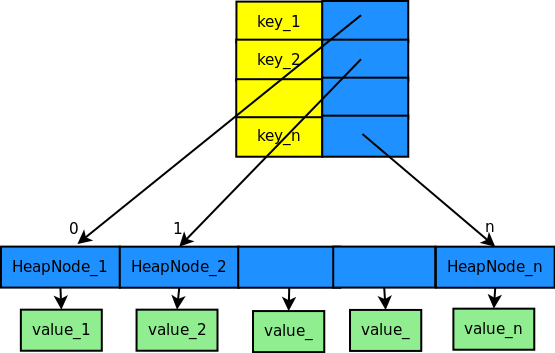
\includegraphics[width=0.7\linewidth]{DinamicHeap.png}
\end{figure}

\end{frame}

\begin{frame}
\frametitle{Runing Median (1/2)}

\begin{figure}
        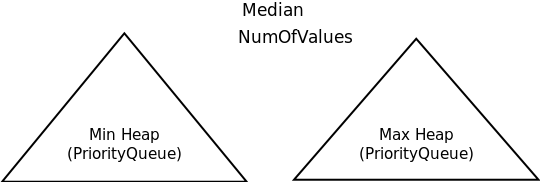
\includegraphics[width=0.8\linewidth]{runningmediang.png}
\end{figure}

\end{frame}


\begin{frame}
\frametitle{Runing Median (2/2)}

\begin{figure}
        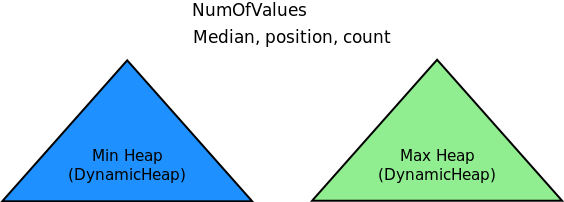
\includegraphics[width=0.8\linewidth]{runningmediand.png}
\end{figure}

\end{frame}

\begin{frame}
\frametitle{Frequent Routes Query}

\begin{algorithm}[H]
\footnotesize
before $\gets$ nodeList.getTopValues()\;
window.add(event)\;
\eIf{ nodeList.containsKey(event.route) }{
        routCount $\gets$ nodeList.get(event.route)\;
        routCount.count++\;
        nodeList.decrementPosition(event.route)\;
}{
        nodeList.add(event.route, new RouteCount(1))\;
}

\While{ there exists expired events }{
        expEvent $\gets$ window.poll()\;
        routCount $\gets$ nodeList.get(expEvent.route)\;
        routCount.count--\;
        \eIf{ routCount.count is 0 }{
                nodelist.remove(expEvent.route)\;
        }{
                nodeList.incrementPosition(expEvent.route)\;
        }
}

now $\gets$ nodeList.getTopValues()\;

\If{ before not equals now }{
        create new top ten route event\;
}

\end{algorithm}


\end{frame}

\begin{frame}
\frametitle{Profitable Cells Query}
\begin{itemize}
        \item Median fare calculation
		\begin{itemize}
			\item Use the PriorityQueue based running median algorithm
		\end{itemize}
        \item Handling empty taxis
		\begin{itemize}
                        \item Generate two events (Pickup event and Drop event) for each dataset event
                \end{itemize}
        \item Handling drop event expiration
		\begin{itemize}
                        \item Keep taxi ids within the profitable cell object
                \end{itemize}
\end{itemize}

\end{frame}


\section{Query evaluation}

\begin{frame}
\frametitle{Sequential Evaluation}

\begin{figure}
        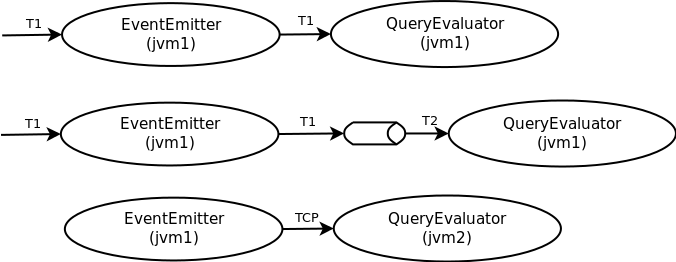
\includegraphics[width=0.8\linewidth]{sequential.png}
\end{figure}

\end{frame}

\begin{frame}
\frametitle{Parallel Evaluation}

\begin{figure}
        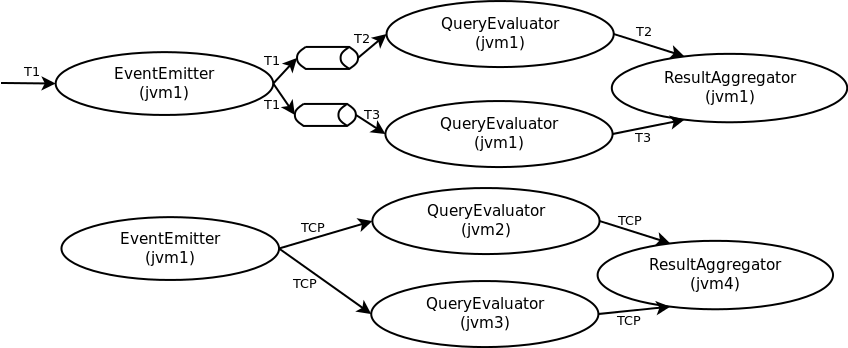
\includegraphics[width=0.8\linewidth]{parallel.png}
\end{figure}

\end{frame}

\begin{frame}
\frametitle{Result Aggregator}

\begin{algorithm}[H]
\footnotesize
before $\gets$ nodeList.getTopValues()\;
\For {key in event.removedKeys}{
        nodeList.remove(key)\;
}

\For {nodeValue in event.newValuesList}{
        \eIf {nodeList.containsKey(nodeValue.key)}{
                existingValue $\gets$ nodeList.get(nodeValue.key)\;
                \eIf { existing value is lesser than current }{
                        update the existing value\;
                        nodeList.decrementPosition(nodeValue.key)\;
                }{
                        update the existing value\;
                        nodeList.incrementPosition(nodeValue.key)\;
                }
        }{
                nodeList.add(nodeValue.key, nodeValue)\;
        }
}

now $\gets$ nodeList.getTopValues()\;
\If { before not equals now }{
        emit new event\;
}

\end{algorithm}

\end{frame}

\section{Experiments}

\begin{frame}
\frametitle{Frequent Routes Query}

\begin{figure}
        \centering
        \begin{subfigure}[b]{0.45\textwidth}
                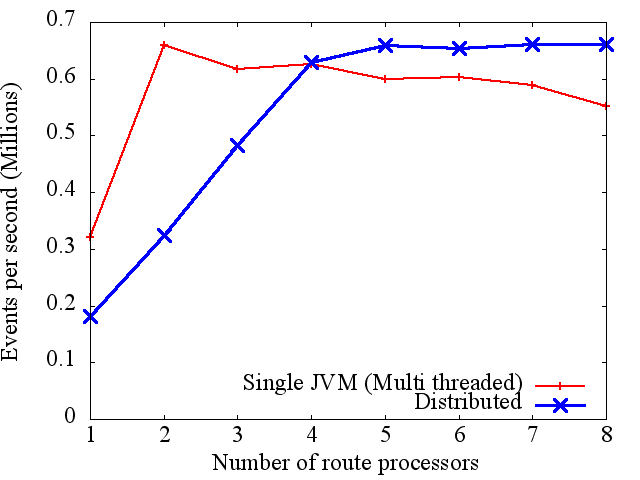
\includegraphics[width=\textwidth]{throughput_route.png}
        \end{subfigure}
        \begin{subfigure}[b]{0.45\textwidth}
                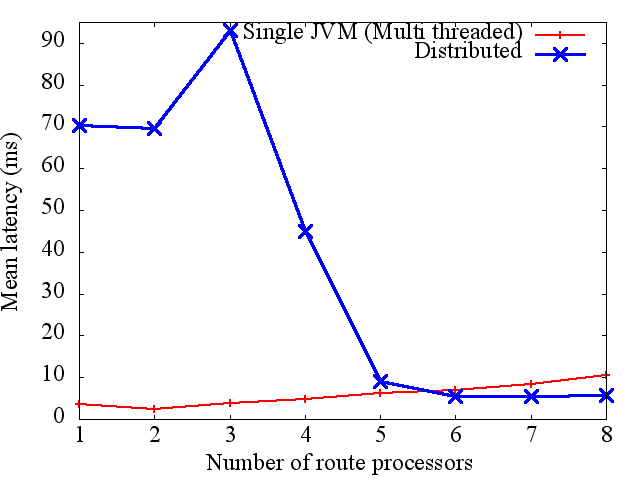
\includegraphics[width=\textwidth]{latency_route.png}
        \end{subfigure}
\end{figure}

\footnotesize For distributed setup throughput increases up to 4 processors while latency remain in a constant after 5 processors. For single JVM setup throughput increases up to 2 nodes and slightly decreases with the number of processors while latency slightly increases with the number of processors.
 

\end{frame}

\begin{frame}
\frametitle{Profitable Cells Query}

\begin{figure}
        \centering
        \begin{subfigure}[b]{0.45\textwidth}
                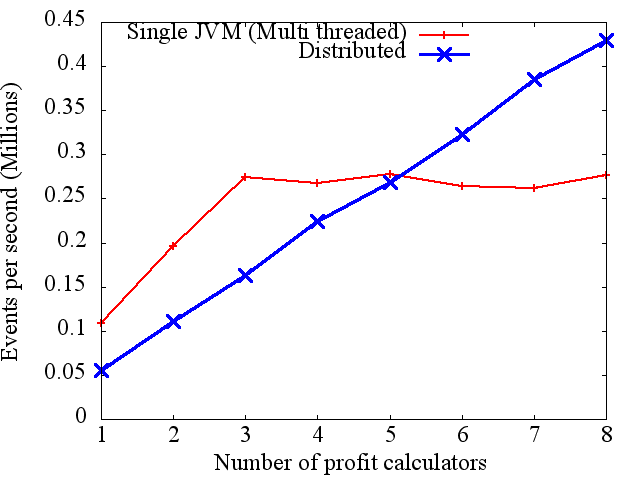
\includegraphics[width=\textwidth]{throughput_profit.png}
        \end{subfigure}
        \begin{subfigure}[b]{0.45\textwidth}
                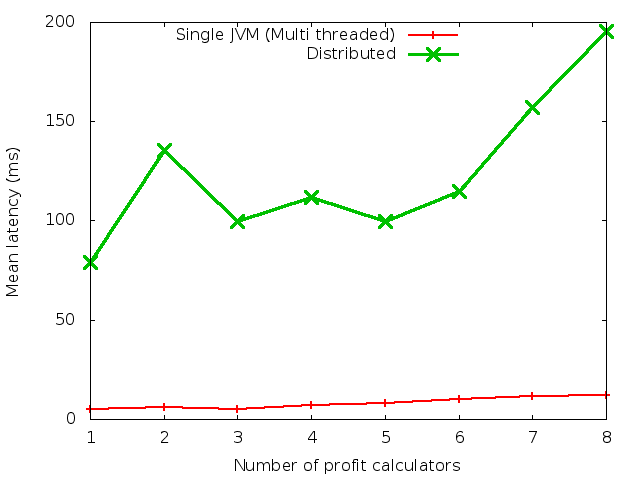
\includegraphics[width=\textwidth]{latency_profit.png}
        \end{subfigure}
\end{figure}

\footnotesize For distributed set up throughput linearly increases and latency increases with higher number of calculators. For single JVM set up throughput linearly increases up to 3 instances and latency slightly increases with the number of calculators. 

\end{frame}

\begin{frame}
\frametitle{Scalability with Window Size}

\begin{figure}
        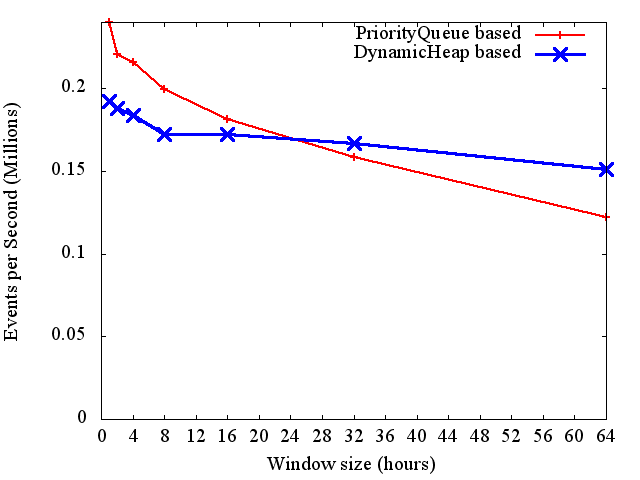
\includegraphics[width=0.6\linewidth]{window.png}
\end{figure}

\footnotesize Both implementations scale even for 64h windows. DynamicHeap based algorithm performs better at higher window sizes.

\end{frame}

\section{Conclusion}

\begin{frame}
\frametitle{Conclusion}
\begin{itemize}
        \item Our queries execute with O(log n) time complexity and hence scale with window size.
        \item Our partitioning technique can be used to scale up the system while producing the desired results. 
	\item We propose an algorithm to find the running median with O(log n) time complexity.
\end{itemize}

\end{frame}

\end{document} 
